\section{Experimental Results \& Discussion}
We evaluated Belief-Based JAL across five independent random seeds in two regimes: against a stationary \texttt{Random} opponent and in \texttt{Self-Play} against an identical learner. Figure~\ref{fig:marl_plot} summarizes outcome percentages across all completed episodes (including draws), whereas Table~\ref{tab:marl_results} normalizes win rates over decisive games only (excluding draws) to match the evaluation convention of Littman~\cite{littman1994markov}.

\begin{table}[htbp]
    \centering
    \scriptsize
    \setlength{\tabcolsep}{4.5pt}
    \caption{Evaluation over $10^5$ steps excluding draws (decisive games only): Belief-Based JAL (5-seed mean) compared with selected benchmarks from Littman~\cite{littman1994markov}.}
    \label{tab:marl_results}
    \begin{tabular}{lllcc}
        \toprule
        \textbf{Algorithm}                     & \textbf{Training} & \textbf{Test} & \textbf{Games} & \textbf{\% won} \\
        \midrule
        Minimax-Q~\cite{littman1994markov}     & Random            & Random        & 6500           & 99.3            \\
        Minimax-Q~\cite{littman1994markov}     & Identical         & Q-best        & 4400           & 37.5            \\
        \midrule
        Independent-Q~\cite{littman1994markov} & Random            & Random        & 11300          & 99.4            \\
        Independent-Q~\cite{littman1994markov} & Identical         & Q-best        & 1200           & 0.0             \\
        \midrule
        \textbf{Belief JAL (Ours)}             & Random            & Random        & \textbf{7323}  & \textbf{99.2}   \\
        \textbf{Belief JAL (Ours)}             & Identical         & Identical     & \textbf{4975}  & \textbf{50.2}   \\
        \bottomrule
    \end{tabular}
\end{table}


\begin{figure}[t]
    \centering
    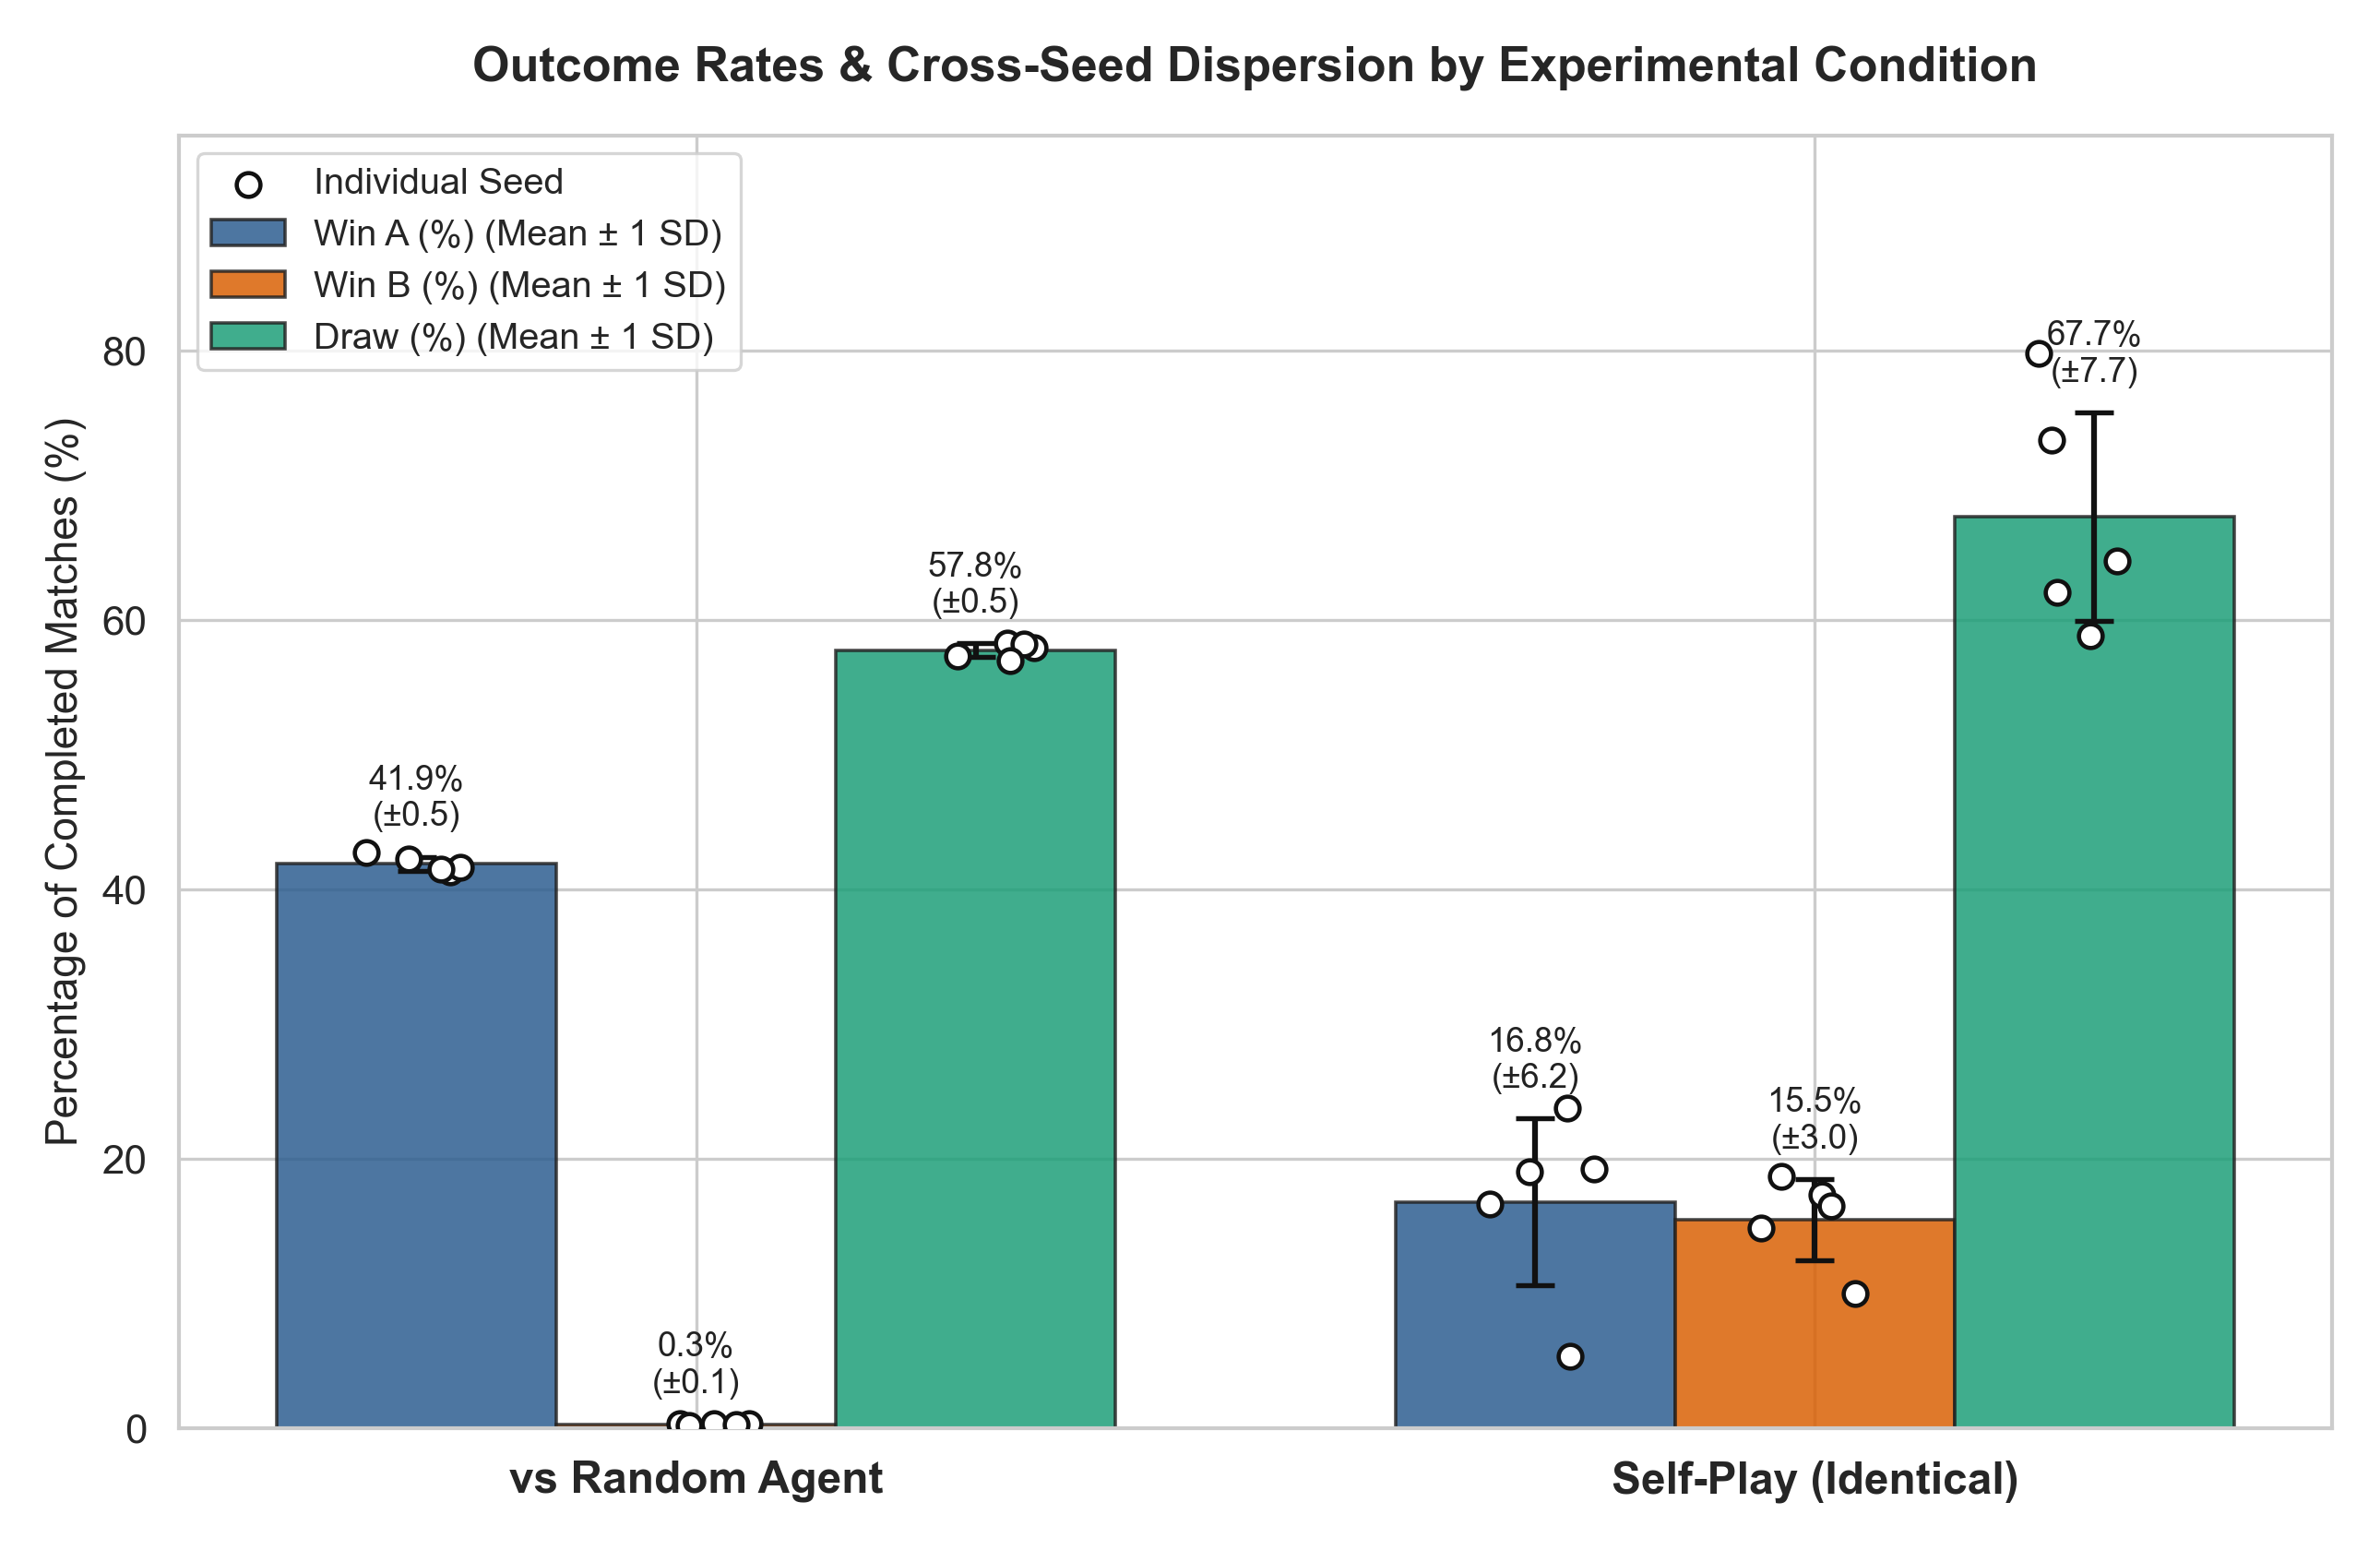
\includegraphics[width=0.96\linewidth]{figures/01_outcome_rates_variance.png}
    \caption{Outcome rates (including draws) and cross-seed dispersion ($\text{Mean} \pm 1\,\text{SD}$ and individual seeds) across regimes.}
    \label{fig:marl_plot}
\end{figure}

Against the stationary \texttt{Random} opponent, the environment reduces to a stationary MDP: the learner converges reliably to an effective offensive policy with minimal cross-seed variance ($41.91\% \pm 0.53\%$ wins, $0.32\% \pm 0.05\%$ losses, $57.78\% \pm 0.50\%$ draws). Excluding draws, Player $A$ achieves a **$99.2\%$** decisive win rate over $7323$ games, closely matching both the win rate ($99.3\%$) and decisive game pace ($6500$--$7200$) of \texttt{Minimax-Q} in~\cite{littman1994markov}.

In \texttt{Self-Play}, aggregate averages confirm structural symmetry between the two learners ($16.82\% \pm 6.19\%$ for $A$ vs.\ $15.49\% \pm 3.02\%$ for $B$, corresponding to $50.2\%$ decisive wins for $A$). However, Figure~\ref{fig:marl_plot2} exposes substantial cross-seed volatility and \emph{path dependence} caused by non-stationarity: standard deviation increases more than tenfold compared to the stationary regime, and early stochastic symmetry breaking can favor either player depending on the seed (e.g., Seed $20$ favors $A$ at $23.8\%$ vs.\ $17.4\%$, whereas Seed $30$ reverses in favor of $B$ at $5.3\%$ vs.\ $14.9\%$).

\begin{figure}[t]
    \centering
    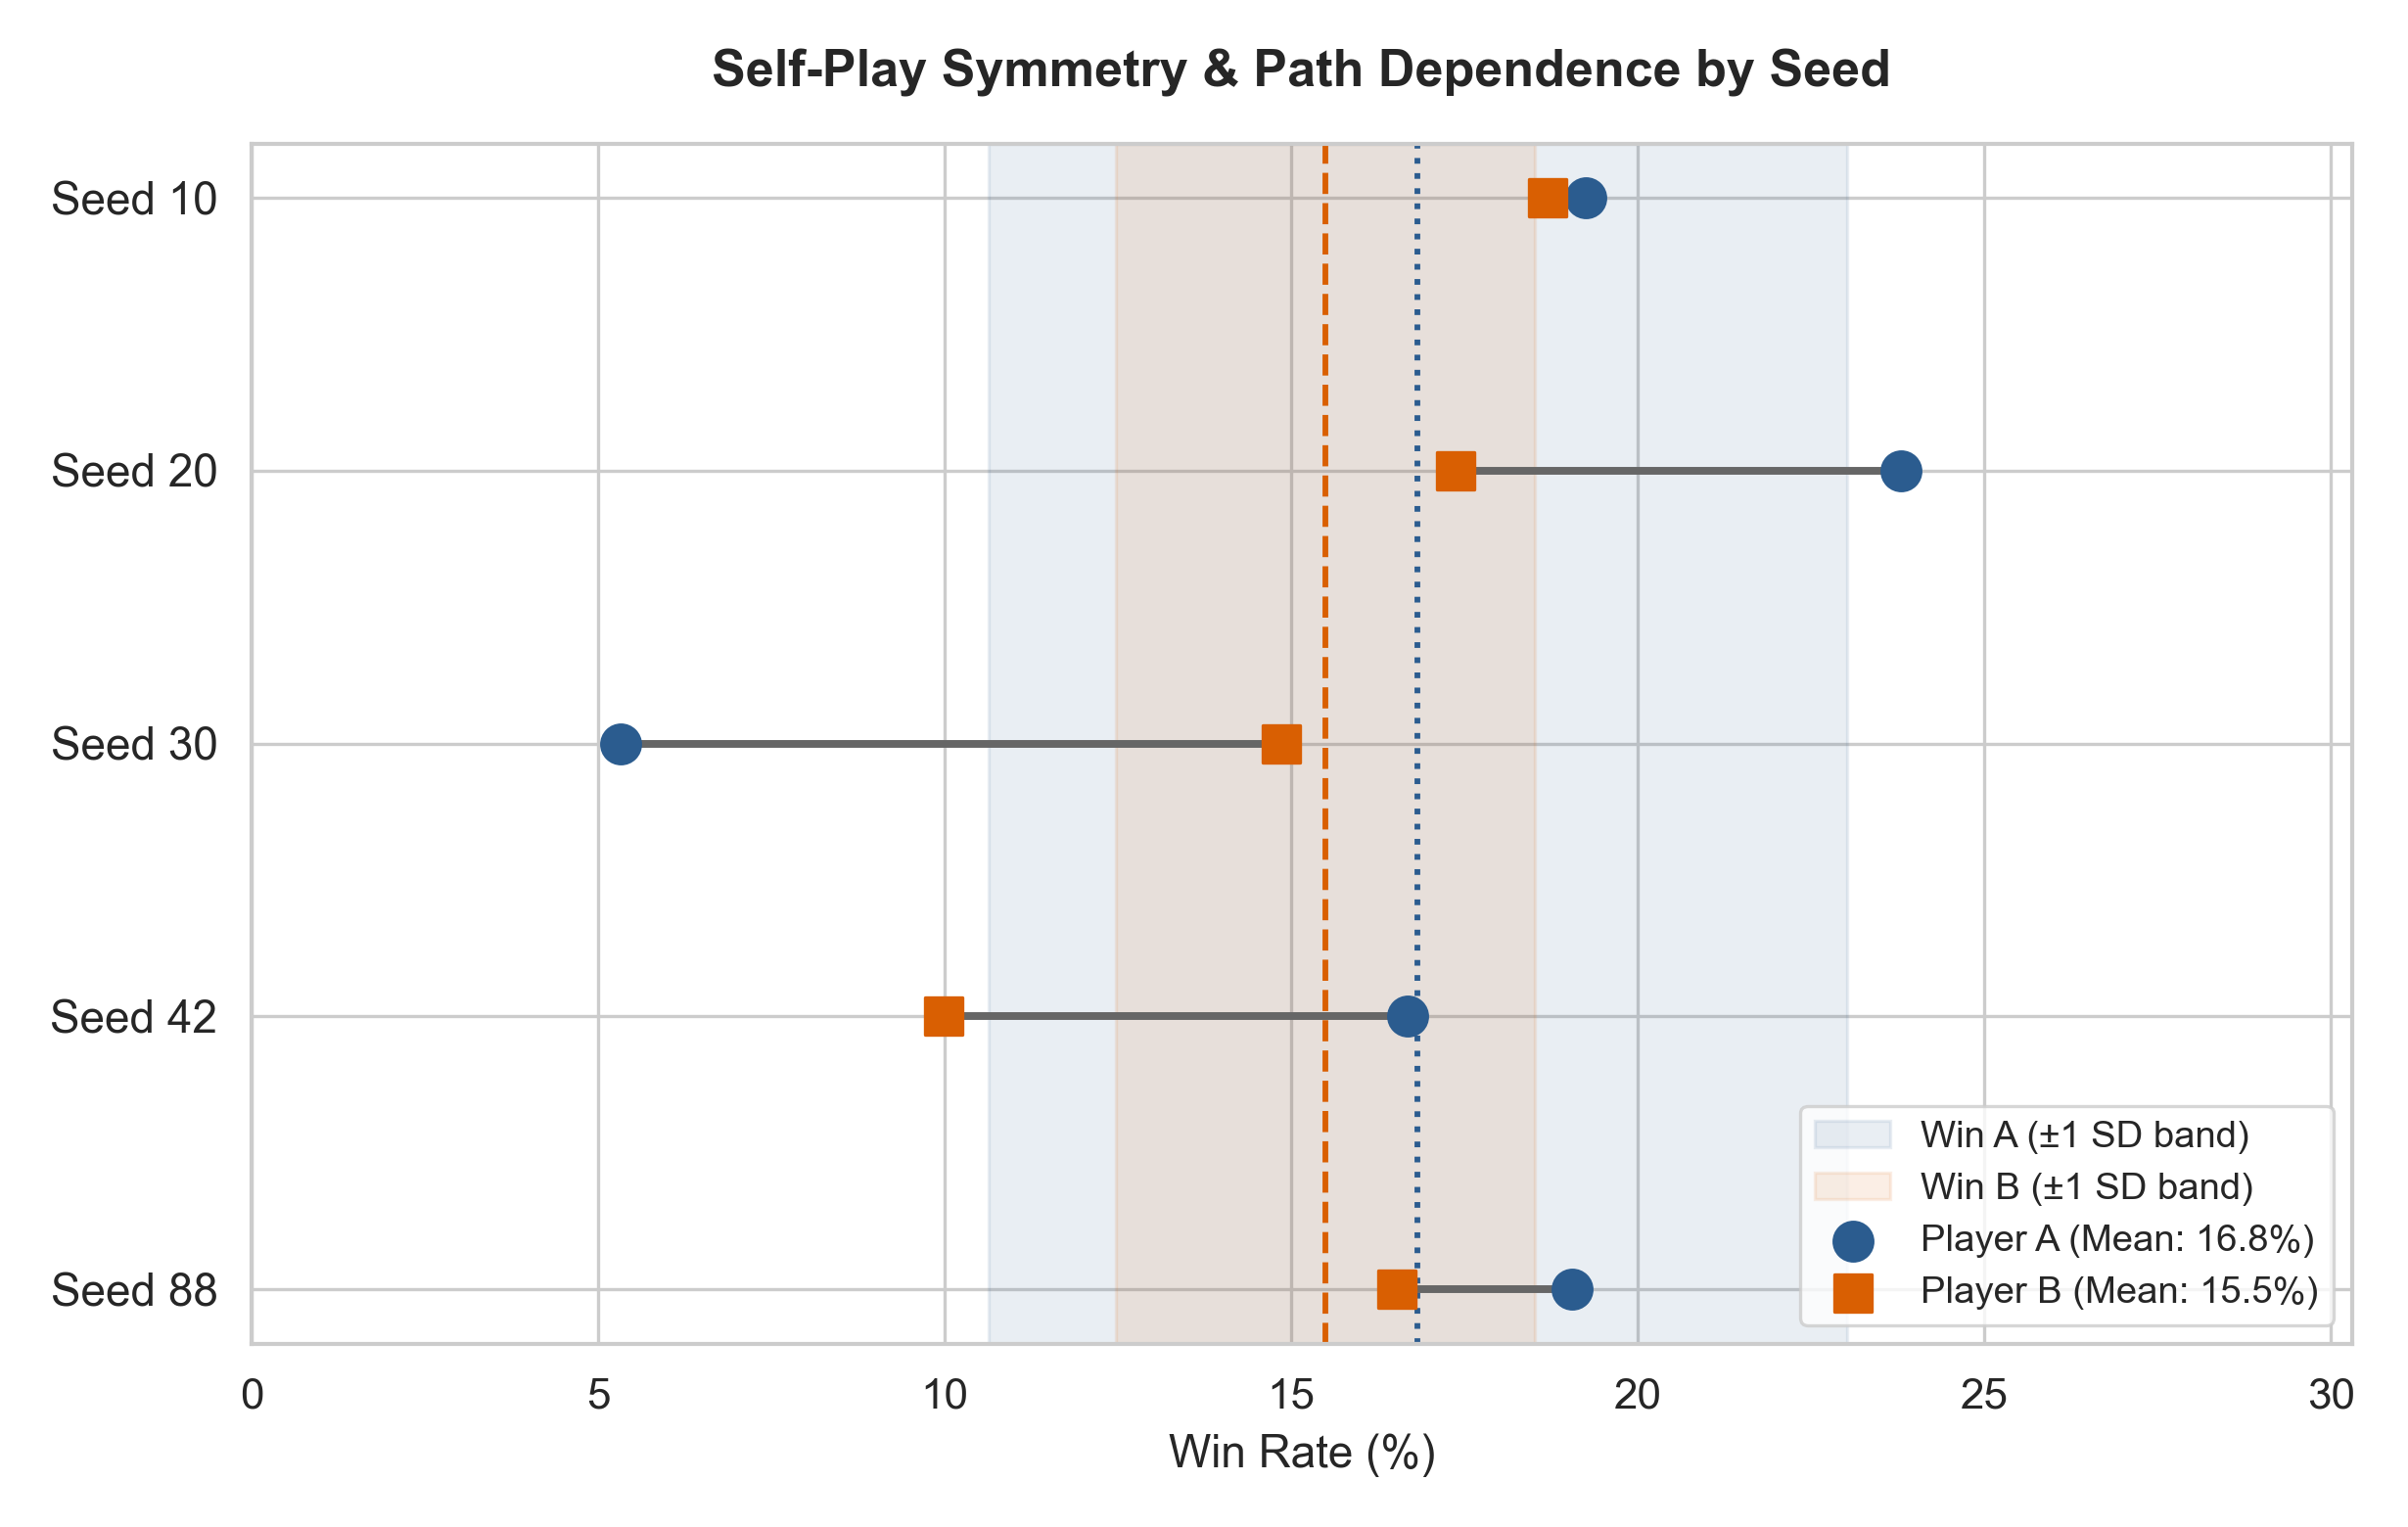
\includegraphics[width=0.96\linewidth]{figures/03_self_play_seed_dynamics.png}
    \caption{Per-seed win rates for Player $A$ and Player $B$ in \texttt{Self-Play}, illustrating symmetry in mean alongside path dependence.}
    \label{fig:marl_plot2}
\end{figure}

Finally, comparing \texttt{Self-Play} with Littman's \texttt{Q-best} benchmarks highlights a key theoretical limitation. Because greedy evaluation ($\epsilon = 0$) induces a \emph{deterministic} policy rather than a mixed strategy equilibrium (as in \texttt{Minimax-Q}), two identical deterministic learners frequently lock into front-to-front stalemates—raising draws from $57.8\%$ to $67.7\%$—and, like \texttt{Independent-Q} ($0.0\%$ vs.\ \texttt{Q-best}), remain inherently exploitable by a dedicated best-response adversary.
